\documentclass[conference]{IEEEtran}
\IEEEoverridecommandlockouts
\usepackage{cite}
\usepackage{amsmath,amssymb,amsfonts}
\usepackage{algorithmic}
\usepackage{graphicx}
\usepackage{textcomp}
\usepackage{overpic}
\usepackage{xcolor}
\usepackage{hyperref}
\def\BibTeX{{\rm B\kern-.05em{\sc i\kern-.025em b}\kern-.08em
    T\kern-.1667em\lower.7ex\hbox{E}\kern-.125emX}}
\newcommand\todo[1]{\textcolor{red}{TODO #1}}

\begin{document}

\title{Virtual Neurorobotics in the Human Brain Project}
\author{Max Becker, Olivier Boder and Qianlin Wu\\FZI Forschungszentrum Informatik\\Karlsruhe, Germany}

\maketitle
\thispagestyle{plain}
\pagestyle{plain}

\begin{abstract}
In this paper the challenge for the neurorobotics praktikum is presented and some solutions are discussed.
The challenge and some theoretic background are explained in the beginning followed by the attempted solutions.
The first solution is a hard-coded throw and the second one a learning approach using evolutionary algorithms and spiking neural networks.
\end{abstract}


\begin{IEEEkeywords}
Spiking Neural Networks, Evolutionary Algorithms, Neurorobotics Platform, Human Brain Project
\end{IEEEkeywords}


% !TEX root = ../Ausarbeitung.tex
\section{Introduction}
In scope of the \textit{Praktikum} within the Human Brain Project, we work with the Neurorobotics Platform (NRP) which provides a simulation environment for robotics.
More specifically, our experiment setup consists of a table, on which a robot arm is placed.
The robot arm has six joints and a hand with five fingers.
In front of the robot arm, a cylinder is placed on the table.
The goal of the Praktikum is to move the cylinder as far as possible with the robot arm.
This can be performed by just hitting the cylinder away or by grabbing the cylinder and throwing it as far as possible.
The performance is measured by the distance of the cylinder from the table.
In the following, several strategies to fulfil this task are presented.
These consist in a hard-coded approaches and in more sophisticated approaches using learning algorithms.
The setup is depicted in \autoref{fig:hbbprak_2018}.

\begin{figure}[h]
\centering
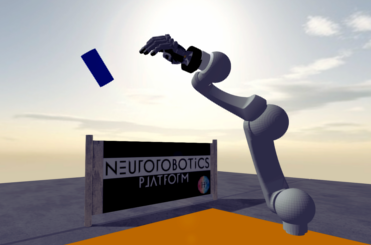
\includegraphics[width=.95\columnwidth]{figures/hbpprak_2018.png}
\caption{The goal is to throw the cylinder as far as possible.}
\label{fig:hbbprak_2018}
\end{figure}
% !TEX root = ../Ausarbeitung.tex
\section{Evolutionary Algorithms}
\label{sec:ea}
Evolutionary algorithms are inspired by nature and evolution.
They try to approximate a solution following the principle of survival of the fittest.
In fact, an evolutionary algorithm models a population consisting of several individuals.
Each individual represents a solution to a task, such as an optimization problem, and is evaluated by a fitness function.
One populations is called a generation.
The elite of each generation, i.e. the individuals performing best according to their fitness, is then selected to evolve the next generation.
This allows the population to evolve towards better solutions.
The evolution of a population corresponds to the mutation of individuals.
The evolution process is depicted in \autoref{fig:ea}.

\begin{figure}[h]
\centering
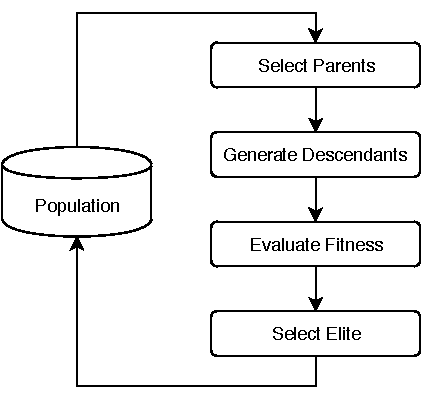
\includegraphics[width=.7\columnwidth]{figures/ea_fig.pdf}
\caption{An illustration of an evolutionary algorithm learning. \cite{Dillmann2017}}
\label{fig:ea}
\end{figure}

To mutate individuals, the crossover strategy can be applied.
Crossover is used to generate new offspring by combining the genetic information of two parents.
One way to combine their genetic information is single-point crossover.
The genetic sequences of both parents are split at a randomly chosen point.
The second part, i.e. the tail, is then swapped between the parents.
Hence, each new individual has its first parents genetic information until the chosen point, followed by the genetic sequence of the other parent.
To apply more variety into the recombination of the genetic information k-point crossover can be applied.
Instead of only one point, more such random points are picked in the sequence, at which alternately information is swapped between the parents.
\cite{Dillmann2017}

As individuals are evolving over generations, they may improve their fitness and thus optimize a solution for the task.
Their genetic information can therefore be parameters to solve a problem.
Overall, there is no specific or correct parameter assumption needed for initialization, as they will be approximated by evolving over generations.

\section{Spiking Neural Networks}
Spiking neural networks try to mimic natural neural networks more closely than other artificial neural networks.
The neurons in spiking neural networks are connected via synapses in a directed graph.
Every neuron in the network has a membrane potential.
If this potential exceeds a certain threshold the neuron fires meaning it sends a spike to all its succeeding neurons in the network.
The potential of the spiking neuron is then reset and it enters a small refractory period in which it can't fire again.
If a neuron receives a spike from a predecessor its membrane potential rises or falls depending on the synaptic weight, in the periods between spikes the neurons leeks some of their potential.
To learn with a spiking neural network the weights of the synapses are changed.
These weights determine how much influence a spike has on the potential of a succeeding neuron.
In contrast to other artificial neural networks the neurons don't have to be organized in strict layers and not all neurons in a layer need to be computed at the same time.
The information is less encoded in the neurons values and more in the timing of the spikes.
However it is harder to learn with spiking neural networks because the spikes aren't differentiable which means you can't learn using backpropagation.
One possibility to learn the weights are evolutionary algorithms.
% !TEX root = ../Ausarbeitung.tex
\section{Hard-coded Approach}
\label{sec:hard-coded}
In the hard-coded approach various states are defined each corresponding to a pose of the robot arm.
A state machine cycles through these states and sends control messages to two scripts controlling the robot.
The positions are initially determined empirically and later generalised with a set of equations to enable the robot to grab the cylinder from different positions on the table.

\subsection{State Machine}
\autoref{fig:statemachine} shows the 5 states used to control the robots movement: \textit{Approach}, \textit{Grasp}, \textit{Prepare}, \textit{Throw} and \textit{Release}.
The first two states let the robot approach and grasp the cylinder.
In \textit{Prepare} the robot reaches back to prepare for its throw.
In the last two states the robot executes the actual throwing motion and finally releases the cylinder.
Each time a new state is reached, the state machine sends a message via ROS to the respective control script: \textit{Hand Control} or \textit{Arm Control}.
These control scripts then choose a configuration according to the current state and adjust the robots pose.

\begin{figure}[tpb]
\centering
	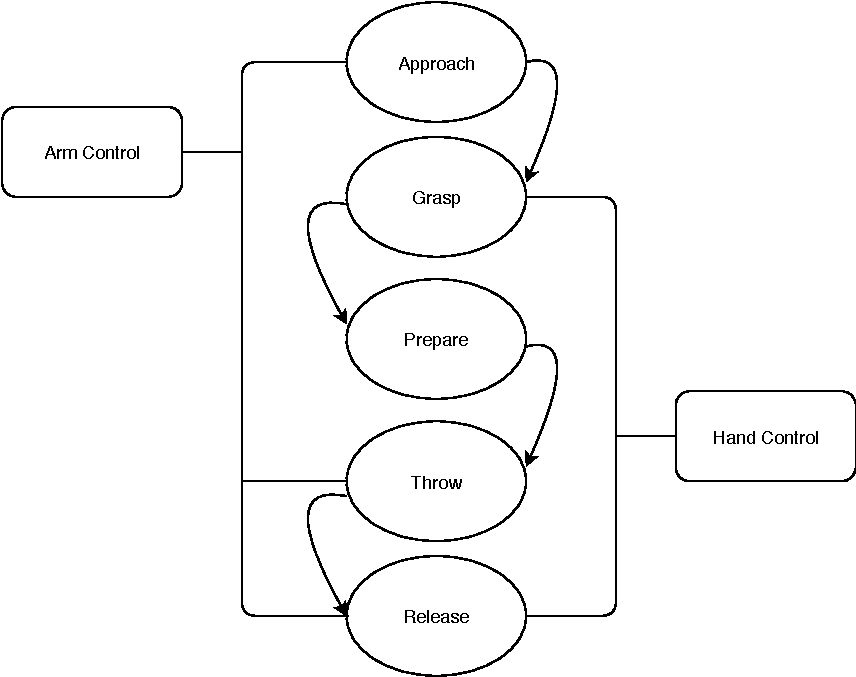
\includegraphics[width=0.96\linewidth]{figures/state.pdf} 
	\caption{The state machine controls the behavior of the robot.}
	\vspace{-0.4cm}
	\label{fig:statemachine}
\end{figure}

\subsection{Inverse Kinematics}
To grab the cylinder from different positions on the table, the robots inverse kinematics are used to determine the joint angles.
When a new cylinder is spawned in the simulation, its position gets published to a ROS topic.
If the cylinder position is $(C_x, C_y, C_z)$ and the robots position is $(R_x, R_y, R_z)$, the angle $\alpha$ for the first joint (see \autoref{fig:top}) can be calculated as follows:

\begin{equation}
\label{simple_equation}
M_1=\alpha = arctan((C_y-R_y)/(C_x-R_x))
\end{equation}

\begin{figure}[htpb]
\centering
	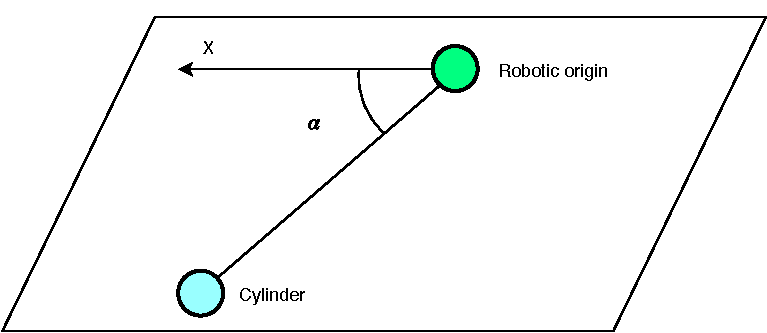
\includegraphics[width=0.96\linewidth]{figures/top_view.pdf} 
	\caption{The platform with the robot arm and the cylinder seen from above.}
	\vspace{-0.4cm}
	\label{fig:top}
\end{figure}

Using the empirically determined configuration for the initial hard-coded grasp, the length of the robot arm segments \textit{Arm\_2} and \textit{Arm\_4} can be calculated.
For reference see \autoref{fig:right}.

\begin{equation}
\begin{aligned}
\delta=2*\pi-\beta-\gamma\\
c=\sqrt{(R_x-C_x)^2+(R_y-C_y)^2}\\
\textit{Arm\_2}=c*sin(\gamma)/sin(\delta)\\
\textit{Arm\_4}=c*sin(\beta)/sin(\delta)\\
\end{aligned}
\end{equation}

With the lengths of the arm segments now known, the remaining angles can be computed using \autoref{eq:config}.
The angles for the third and fifth joint are $0$.

\begin{equation}
\label{eq:config}
\begin{aligned}
M_2=\beta=arccos((a^2+c^2-b^2)/2*a*c)\\
M_4=\pi-\delta=\pi-arccos((a^2+b^2-c^2)/2*a*b)\\
M_6=\gamma=arccos((b^2+c^2-a^2)/2*b*c)\\
\textbf{with}\ c=\sqrt{(R_x-C_x)^2+(R_y-C_y)^2}
\end{aligned}
\end{equation}

\begin{figure}[tpb]
\centering
	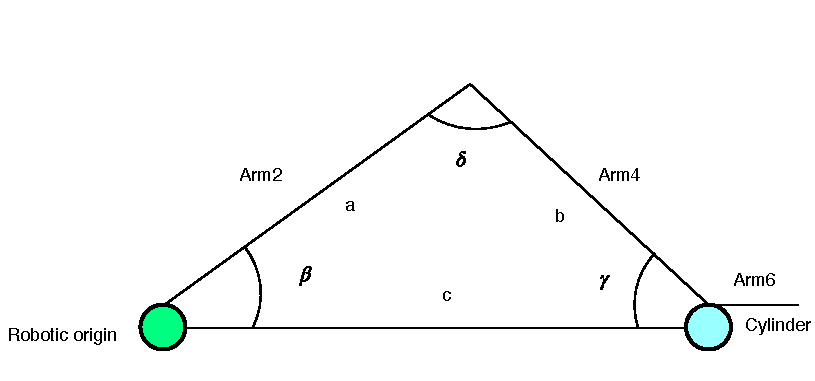
\includegraphics[width=0.96\linewidth]{figures/right_v.pdf} 
	\caption{The platform with the robot arm and the cylinder seen from the side.}
	\vspace{-0.4cm}
	\label{fig:right}
\end{figure}




% !TEX root = ../Ausarbeitung.tex
\section{Learned Approaches}
The next approach was trying to learn some of the movements instead of hard-coding them.
We used an evolutionary approach to learn weights for a spiking neural network which controls the robots movements.

\subsection{Evolutionary Approach}
In this approach the robot is controlled by a spiking neural network which can be seen in \autoref{fig:network}.
The network has three input and seven output neurons which are fully connected.
The three dimensional position of the cylinder is used for the input neurons.
Six of the output neurons control the six joints of the robots arm and the last neuron controls when the hand should release the cylinder.
The position values of the cylinder are directly

The individuals of our evolutionary algorithm are lists of 21 values each representing one weight of the network.
To evaluate the individuals a throw is simulated and the distance of the cylinder from the table represents the fitness of the individual.
After each individual of a generation is evaluated we select the elite which consists of the best 50\% of the individuals.
The elite gets copied into the next generation and the remaining individuals are generated by mutating the individuals of the elite.

\begin{figure}[h]
\centering
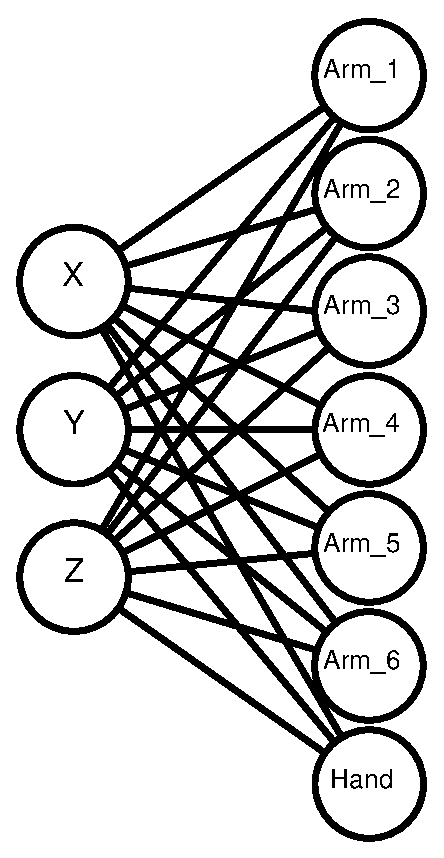
\includegraphics[width=.5\columnwidth]{figures/net.eps}
\caption{Network architecture.}
\label{fig:network}
\end{figure}

\subsubsection{Mutation Strategies}
Three different mutation strategies were implemented to generate new descendants.
The first method uses only one parent and adds or subtracts small random values from its weights.
The other two methods use two parents.
One was a single-point crossover at a random position meaning you take the first n weights from one parent and the remaining ones from the second one.
The last method is a k-point crossover.
At each position this method chooses randomly one of the parents weights.

\subsection{Simplified Problem}
As our first learned approach wasn't really successful we try to reduce the search space for the evolutionary algorithm.
To achieve this we restrict which joints the robot could use to execute the throw.
We fix all rotational joints by setting the respective weights in the neural network to zero because this probably won't impact the robots ability to make a good throw very much.
This reduces the number of weights to be learned from 21 to 12.
% !TEX root = ../Ausarbeitung.tex
\section{Problems}\label{sec:problems}
While working on the challenge some problems arose with the neurorobotics platform itself as well as the server infrastructure around it.
The simulations in the neurorobotics platform are non-deterministic which leads to non-reproducible results.
This non-determinism probably results from floating point inaccuracy.
In addition to that the grasping of the cylinder is very unreliable.
If the cylinder is grasped too tightly the robot starts shaking, sometimes resulting in the hand exploding and the cylinder flying huge distances (see \autoref{fig:dispersed}).
In some extreme cases the hole table the robot is mounted to moves, which results in the grasping not working afterwards due to a change in the relation of the robot and world coordinate systems.
There were also problems with the platform crashing regularly because of different reasons.
All these problems occurred on the server install of the platform.
In absence of a working local install it wasn't possible to check if they were specific to the server install or the platform itself.

\begin{figure}[h]
\centering
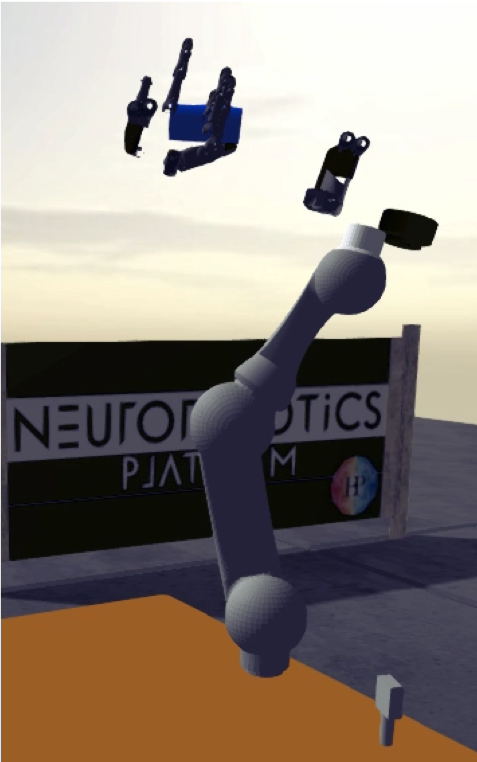
\includegraphics[width=.95\columnwidth]{figures/dispersed_robot.png}
\caption{Occasionally, different parts of the robot scatter.}
\label{fig:dispersed}
\end{figure}
\section{Results}
We enabled the robot to grasp the cylinder at random positions and throw it using a set of synaptic weights generated by the evolutionary algorithm.
However the problems described in \autoref{sec:problems} make it very hard to learn anything.
The individuals of the evolutionary algorithm can execute throws but due to glitches in the simulation, like the shaking hand, the measured distance is not representative for the quality of the movement.
In addition the non-determinism in the simulation makes it hard to compare the results as the same individual gets different distances if executed multiple times.
That results in the algorithm not really learning anything and evolving the weights rather randomly.
% !TEX root = ../Ausarbeitung.tex
\section{Conclusion}
\label{sec:conclusion}
\todo{}
Two different approaches are presented to make the robot arm throw the cylinder.
The first approach controls the robot arm with hard-coded configurations which have been determined empirically.
This not only involves the static movements of the robot, but also grasping the cylinder at random positions reliably which is computed with inverse kinematics.
The second approach aims for a learned solution based on spiking neural networks.
For this purpose, an evolutionary algorithm has been chosen in order to optimize the synaptic weights.
Given the circumstances, various approaches have been implemented that lead to reasonably results.
However, results are not comparable due to non-deterministic behavior.

\subsection{Future Work} % (fold)
\label{sub:future_work}
\todo{}
Having set a basis for learning the networks parameters, different population sizes and numbers of generations with different mutation strategies could be compared in the evolutionary algorithm.
Moreover, finding a good set of initial synaptic weights could help to converge faster towards a desired solution.
However, unconventional solutions, such as fast and wild spinnings of the robot, that don't look like natural and realizable throwing movements, may, in that case, not be among the solutions.
To further reduce the number of parameters, it could be considerable to use only the y coordinate of the cylinder as an input, assuming that the cylinder is thrown in y direction.
In order to not only learn the throwing sequence, the grasping part could also be learned.
The learning process in general could be supported by other inputs such as cameras or haptic sensors, but these would again increase the number of parameters to be learned.
Finally, artificial neural networks could be used for learning in comparison to evolutionary algorithms.

% subsection future_work (end)



\begin{thebibliography}{00}
\bibitem{b1} A. Tavanaei, M. Ghodrati, S. Kheradpisheh, ``Deep Learning in Spiking Neural Networks``
\bibitem{b2} F. Ponulak, A. Kasinski, ``Introduction to spiking neural networks: Information processing, learning and applications.``
\bibitem{b3} Z. Bing, C.Meschede, F. R{\"o}hrbein, ``A Survey of Robotics Control Based on Learning-Inspired Spiking Neural Networks``
\bibitem{Dillmann2017} R. Dillmann, J. M. Z{\"o}llner, ``Machine Learning 1 - Basic Methods'', lecture 14, 2017


\end{thebibliography}



\end{document}
